% !TeX program = xelatex
% Build with: pnpm paper:build:zh
% The build target runs XeLaTeX and BibTeX to completion and verifies citations.
\documentclass[manuscript,nonacm]{acmart}

\usepackage[UTF8,fontset=fandol,scheme=plain]{ctex}
\usepackage{booktabs}
\usepackage{tabularx}
\usepackage{array}
\usepackage{xcolor}
\usepackage{graphicx}
\usepackage{listings}
\usepackage{microtype}
\usepackage{tikz}
\usetikzlibrary{arrows.meta,calc,shapes.geometric}
% Shared publication figure style.
% Keep typography semantic so it follows the active paper template.
% Sizes below are specified for the final figure, before any outer resize.

\definecolor{paiUser}{HTML}{2F5D8A}
\definecolor{paiUserLight}{HTML}{E9F1F8}
\definecolor{paiAgent}{HTML}{A34A3A}
\definecolor{paiAgentLight}{HTML}{F8ECE8}
\definecolor{paiDecision}{HTML}{397261}
\definecolor{paiDecisionLight}{HTML}{E7F2EE}
\definecolor{paiBorder}{HTML}{C9CDD2}
\definecolor{paiNeutral}{HTML}{68717A}
\definecolor{paiPanel}{HTML}{FAFAF8}
\definecolor{paiRevision}{HTML}{B3261E}

\newcommand{\paiFigureFont}{\sffamily\fontsize{8.25}{9.9}\selectfont}
\newcommand{\paiPanelTitleFont}{\sffamily\bfseries\fontsize{9}{10.8}\selectfont}
\newcommand{\paiSecondaryFont}{\sffamily\fontsize{7.5}{9}\selectfont}
\newcommand{\paiAvatarFont}{\sffamily\bfseries\fontsize{7}{8.4}\selectfont}

\tikzset{
  pai-figure/.style={
    x=1cm,
    y=1cm,
    font=\paiFigureFont
  },
  pai-panel/.style={
    rounded corners=5pt,
    fill=paiPanel,
    draw=paiBorder,
    line width=0.55pt
  },
  pai-panel-title/.style={
    font=\paiPanelTitleFont
  },
  pai-chat-surface/.style={
    rounded corners=4pt,
    fill=white,
    draw=paiBorder,
    line width=0.55pt
  },
  pai-user-message/.style={
    rounded corners=3pt,
    draw=paiUser,
    fill=paiUserLight,
    line width=0.7pt,
    minimum height=0.46cm,
    inner xsep=5pt,
    inner ysep=3pt,
    align=center
  },
  pai-agent-message/.style={
    rounded corners=3pt,
    draw=paiAgent,
    fill=paiAgentLight,
    line width=0.7pt,
    minimum height=0.46cm,
    inner xsep=5pt,
    inner ysep=3pt,
    align=center
  },
  pai-user-avatar/.style={
    circle,
    draw=paiUser,
    fill=paiUser,
    text=white,
    line width=0.6pt,
    minimum size=0.46cm,
    inner sep=0pt,
    font=\paiAvatarFont
  },
  pai-agent-avatar/.style={
    circle,
    draw=paiAgent,
    fill=paiAgent,
    text=white,
    line width=0.6pt,
    minimum size=0.46cm,
    inner sep=0pt,
    font=\paiAvatarFont
  },
  pai-secondary/.style={
    text=paiNeutral,
    font=\paiSecondaryFont
  },
  pai-divider/.style={
    densely dotted,
    draw=paiBorder,
    line width=0.55pt
  },
  pai-silence-span/.style={
    densely dotted,
    draw=paiNeutral,
    line width=0.65pt
  },
  pai-user-event/.style={
    rounded corners=2pt,
    draw=paiUser,
    fill=paiUserLight,
    line width=0.7pt,
    minimum width=0.78cm,
    minimum height=0.45cm,
    inner sep=2pt
  },
  pai-agent-event/.style={
    rounded corners=2pt,
    draw=paiAgent,
    fill=paiAgentLight,
    line width=0.7pt,
    minimum width=0.78cm,
    minimum height=0.45cm,
    inner sep=2pt
  },
  pai-pending-event/.style={
    rounded corners=2pt,
    draw=paiAgent,
    fill=white,
    dashed,
    line width=0.8pt,
    minimum width=0.9cm,
    minimum height=0.48cm,
    inner sep=2pt
  },
  pai-plan-group/.style={
    rounded corners=3pt,
    draw=paiDecision,
    fill=paiDecisionLight,
    densely dashed,
    line width=0.6pt
  },
  pai-decision/.style={
    diamond,
    aspect=1.45,
    draw=paiDecision,
    fill=paiDecisionLight,
    line width=0.8pt,
    minimum width=0.65cm,
    minimum height=0.58cm,
    inner sep=1pt
  },
  pai-event-line/.style={
    draw=paiBorder,
    line width=0.45pt
  },
  pai-causal/.style={
    -{Latex[length=1.7mm]},
    draw=paiNeutral,
    line width=0.55pt
  },
  pai-revision/.style={
    -{Latex[length=1.7mm]},
    draw=paiRevision,
    line width=0.7pt
  },
  pai-axis/.style={
    -{Latex[length=1.8mm]},
    draw=paiNeutral,
    line width=0.55pt
  },
  pai-cancel-mark/.style={
    draw=paiRevision,
    fill=white,
    text=paiRevision,
    circle,
    line width=0.7pt,
    minimum size=0.34cm,
    inner sep=0pt,
    font=\paiAvatarFont
  }
}


\setcopyright{none}
\settopmatter{printacmref=false,printccs=false}
\renewcommand\footnotetextcopyrightpermission[1]{}
\pagestyle{plain}
\hypersetup{pdfauthor={Zijie Yang}}

\definecolor{codegreen}{HTML}{164F45}
\definecolor{codecoral}{HTML}{A93428}
\definecolor{codegray}{HTML}{F2EFE8}
\lstdefinelanguage{json}{
  basicstyle=\ttfamily\footnotesize,
  backgroundcolor=\color{codegray},
  breaklines=true,
  columns=fullflexible,
  keepspaces=true,
  showstringspaces=false,
  string=[s]{"}{"},
  stringstyle=\color{codegreen},
  literate=
   *{0}{{{\color{codecoral}0}}}{1}
    {1}{{{\color{codecoral}1}}}{1}
    {2}{{{\color{codecoral}2}}}{1}
    {3}{{{\color{codecoral}3}}}{1}
    {4}{{{\color{codecoral}4}}}{1}
    {5}{{{\color{codecoral}5}}}{1}
    {6}{{{\color{codecoral}6}}}{1}
    {7}{{{\color{codecoral}7}}}{1}
    {8}{{{\color{codecoral}8}}}{1}
    {9}{{{\color{codecoral}9}}}{1}
}
\newcolumntype{Y}{>{\raggedright\arraybackslash}X}
\newcommand{\zhrequirement}[1]{\par\noindent\textbf{#1。}\ }

\title{Proactive AI：从轮次到可重排的对话时间线}

\author{Zijie Yang}
\affiliation{%
  \institution{Airalogy}
  \city{Hangzhou}
  \country{China}
}
\email{yangzijie@airalogy.com}

\begin{abstract}
\textbf{摘要：}
当前的大语言模型聊天通常围绕用户发起的轮次展开：每个请求触发一次回答，
随后系统重新归于静止。人类的异步交流则沿现实时间持续展开，其中包含连续
消息、延迟、沉默、话题重启和主动联系。主动式对话因而不仅需要决定何时发言，
还需要管理尚未执行的对话行动，并允许这些行动随情境变化而修订。
本文提出 Proactive AI，一种以可重排时序消息队列为核心的主动式对话框架。
该框架把交互建模为连续的事件时间线，并把尚未发送的对话行动表示为可修改
的状态。用户事件、对话起搏或预定的决策
时点都可能产生沉默、一条或多条即时消息，或者面向未来的对话行动。系统也
可以在观察到用户消息后暂不产生可见回复，把回复决策推迟到未来。任何计划消息
在实际发送之前都必须根据最新上下文重新判断是否仍适合发送；预定时间的到达
本身并不构成发送依据。
本文进一步给出形式化语义，刻画未来对话行动随上下文变化而更新、撤销和执行
的条件。这一框架使 AI 的参与不再局限于对当前请求的回答，而可以表现为没有
新请求时的主动发起、跨越时间的持续跟进，以及随情境变化而修订的后续行动，
为教育辅导、科学协作与日常陪伴中的长期人机交互提供可执行基础。
\end{abstract}

\ccsdesc[500]{以人为中心的计算~人机交互（HCI）}
\ccsdesc[300]{计算方法~语篇、对话与语用学}
\ccsdesc[300]{软件及其工程~发布订阅／事件驱动架构}

\keywords{主动式 AI，对话智能体，异步对话，混合主动性，时序规划，人机交互}

\begin{document}
\renewcommand{\figurename}{图}
\renewcommand{\tablename}{表}
\renewcommand{\refname}{参考文献}
\renewcommand{\keywordsname}{关键词}
\captionsetup[figure]{name=图}
\captionsetup[table]{name=表}
\maketitle

\section{引言}

大语言模型（large language model，LLM）最常见的交互界面看似非常简单：
用户提交输入，模型产生一个可见的助手轮次，随后系统再次等待用户操作。这种
契约适合问答和命令执行，却无法准确描述异步的社交通信。人在聊天时经常把
一个想法拆成多条消息，集中回应对方连续发来的多条消息，连续发送多个回复，
看到消息后暂不回应、过一段时间再回复，稍后回到先前的话题，或者主动发起
下一段交流（图~\ref{fig:timeline}；附图~\ref{fig:dialogue-patterns}）。

这些现象中，主动发起尤其揭示了轮次式聊天的一项根本限制：一旦用户停止输入，
系统便失去再次参与对话的触发来源。即使双方以“拜拜”结束一次交流，真实的
人际沟通仍可能在稍后由任意一方重新开启；纯粹由用户轮次驱动的系统则会无限期
等待。因此，面向持续交互的主动式系统首先需要在没有新用户输入时重新获得判断
机会。但这仍不足以保证对话能够继续：如果系统在每次判断时都选择沉默，交互仍
可能永久停滞。

\begin{figure*}[t]
  \centering
  \resizebox{0.98\textwidth}{!}{\begin{minipage}{15.9cm}
  \centering
  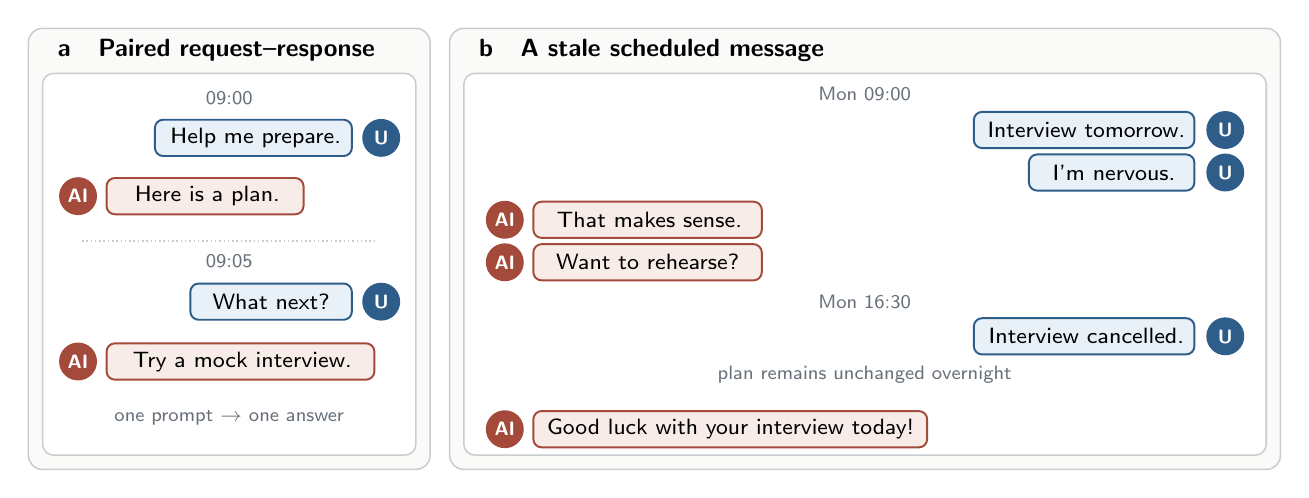
\begin{tikzpicture}[pai-figure]

% (a) A familiar chat interface constrained to paired turns.
\filldraw[pai-panel]
  (0,0.10) rectangle (5.10,5.70);
\node[pai-panel-title, anchor=west] at (0.25,5.42)
  {a\quad Paired request--response};
\filldraw[pai-chat-surface]
  (0.18,0.28) rectangle (4.92,5.13);

\node[pai-secondary] at (2.55,4.81) {09:00};
\node[pai-user-avatar] at (4.48,4.31) {U};
\node[pai-user-message, anchor=east, text width=2.15cm] at (4.12,4.31)
  {Help me prepare.};
\node[pai-agent-avatar] at (0.63,3.57) {AI};
\node[pai-agent-message, anchor=west, text width=2.15cm] at (0.98,3.57)
  {Here is a plan.};

\draw[pai-divider]
  (0.68,3.00) -- (4.42,3.00);
\node[pai-secondary] at (2.55,2.75) {09:05};
\node[pai-user-avatar] at (4.48,2.23) {U};
\node[pai-user-message, anchor=east, text width=1.70cm] at (4.12,2.23)
  {What next?};
\node[pai-agent-avatar] at (0.63,1.47) {AI};
\node[pai-agent-message, anchor=west, text width=3.05cm] at (0.98,1.47)
  {Try a mock interview.};
\node[pai-secondary] at (2.55,0.75)
  {one prompt $\rightarrow$ one answer};

% (b) A concrete failure in which a scheduled message becomes stale.
\filldraw[pai-panel]
  (5.35,0.10) rectangle (15.90,5.70);
\node[pai-panel-title, anchor=west] at (5.60,5.42)
  {b\quad A stale scheduled message};
\filldraw[pai-chat-surface]
  (5.53,0.28) rectangle (15.72,5.13);

\node[pai-secondary] at (10.62,4.87) {Mon 09:00};
\node[pai-user-avatar] at (15.20,4.41) {U};
\node[pai-user-message, anchor=east, text width=2.45cm] at (14.82,4.41)
  {Interview tomorrow.};
\node[pai-user-avatar] at (15.20,3.87) {U};
\node[pai-user-message, anchor=east, text width=1.75cm] at (14.82,3.87)
  {I'm nervous.};
\node[pai-agent-avatar] at (6.05,3.27) {AI};
\node[pai-agent-message, anchor=west, text width=2.55cm] at (6.40,3.27)
  {That makes sense.};
\node[pai-agent-avatar] at (6.05,2.73) {AI};
\node[pai-agent-message, anchor=west, text width=2.55cm] at (6.40,2.73)
  {Want to rehearse?};

\node[pai-secondary] at (10.62,2.23) {Mon 16:30};
\node[pai-user-avatar] at (15.20,1.79) {U};
\node[pai-user-message, anchor=east, text width=2.45cm] at (14.82,1.79)
  {Interview cancelled.};
\draw[pai-silence-span]
  (8.90,1.30) -- (12.34,1.30);
\node[pai-secondary, fill=white, inner xsep=4pt] at (10.62,1.30)
  {plan remains unchanged overnight};
\node[pai-agent-avatar] at (6.05,0.61) {AI};
\node[pai-agent-message, anchor=west, text width=4.65cm] at (6.40,0.61)
  {Good luck with your interview today!};

\end{tikzpicture}


  \vspace{0.12cm}
  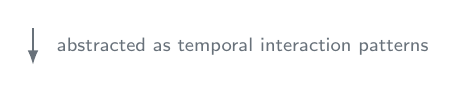
\begin{tikzpicture}[pai-figure]
    \draw[pai-axis]
      (0,0.24) -- (0,-0.22);
    \node[pai-secondary, anchor=west] at (0.18,0.01)
      {abstracted as temporal interaction patterns};
  \end{tikzpicture}
  \vspace{0.04cm}

  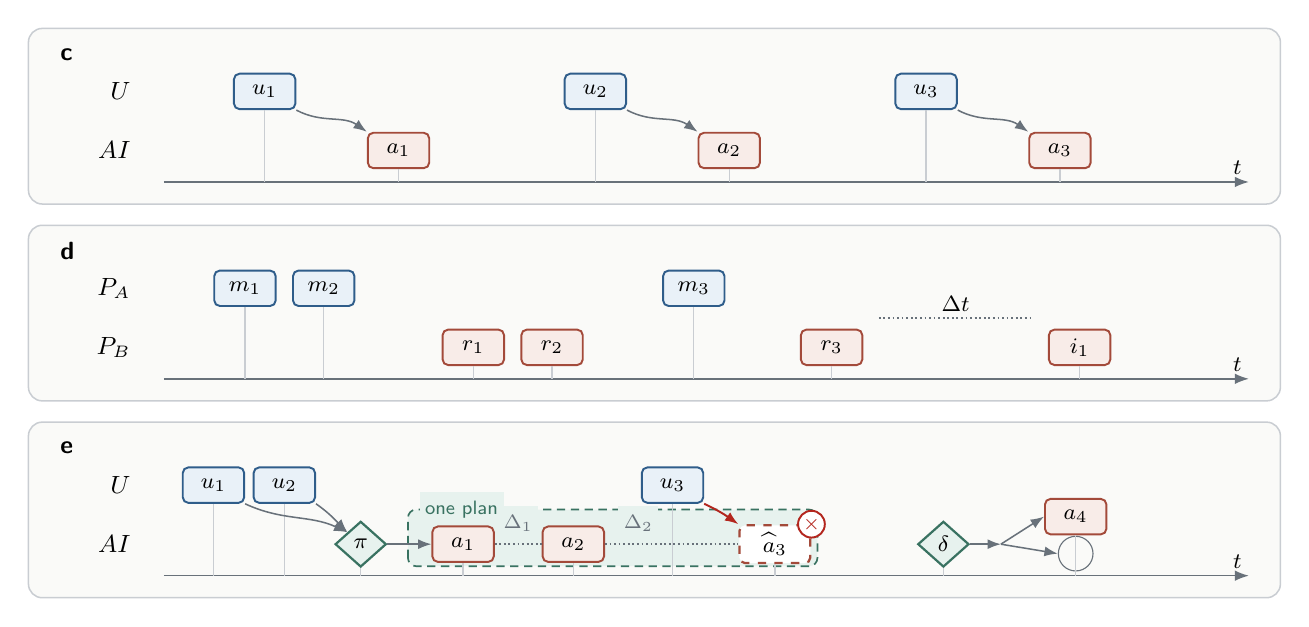
\begin{tikzpicture}[pai-figure]

% (c) Conventional request-response turns.
\filldraw[pai-panel]
  (0,5.02) rectangle (15.9,7.25);
\node[pai-panel-title, anchor=west] at (0.28,6.92) {c};
\node[pai-panel-title, anchor=east] at (1.42,6.45) {$U$};
\node[pai-panel-title, anchor=east] at (1.42,5.70) {$AI$};
\draw[pai-axis] (1.72,5.30) -- (15.50,5.30) node[above left=-1pt] {$t$};

\node[pai-user-event] (a-u1) at (3.00,6.45) {$u_1$};
\node[pai-agent-event] (a-a1) at (4.70,5.70) {$a_1$};
\node[pai-user-event] (a-u2) at (7.20,6.45) {$u_2$};
\node[pai-agent-event] (a-a2) at (8.90,5.70) {$a_2$};
\node[pai-user-event] (a-u3) at (11.40,6.45) {$u_3$};
\node[pai-agent-event] (a-a3) at (13.10,5.70) {$a_3$};
\foreach \n in {a-u1,a-a1,a-u2,a-a2,a-u3,a-a3} {
  \draw[pai-event-line] (\n.south) -- (\n.south |- 0,5.30);
}
\draw[pai-causal] (a-u1.south east) to[out=-28,in=145] (a-a1.north west);
\draw[pai-causal] (a-u2.south east) to[out=-28,in=145] (a-a2.north west);
\draw[pai-causal] (a-u3.south east) to[out=-28,in=145] (a-a3.north west);

% (d) Human asynchronous messaging.
\filldraw[pai-panel]
  (0,2.52) rectangle (15.9,4.75);
\node[pai-panel-title, anchor=west] at (0.28,4.42) {d};
\node[pai-panel-title, anchor=east] at (1.42,3.95) {$P_A$};
\node[pai-panel-title, anchor=east] at (1.42,3.20) {$P_B$};
\draw[pai-axis] (1.72,2.80) -- (15.50,2.80) node[above left=-1pt] {$t$};

\node[pai-user-event] (b-m1) at (2.75,3.95) {$m_1$};
\node[pai-user-event] (b-m2) at (3.75,3.95) {$m_2$};
\node[pai-agent-event] (b-r1) at (5.65,3.20) {$r_1$};
\node[pai-agent-event] (b-r2) at (6.65,3.20) {$r_2$};
\node[pai-user-event] (b-m3) at (8.45,3.95) {$m_3$};
\node[pai-agent-event] (b-r3) at (10.20,3.20) {$r_3$};
\node[pai-agent-event] (b-i1) at (13.35,3.20) {$i_1$};
\foreach \n in {b-m1,b-m2,b-r1,b-r2,b-m3,b-r3,b-i1} {
  \draw[pai-event-line] (\n.south) -- (\n.south |- 0,2.80);
}
\draw[pai-silence-span]
  (10.80,3.57) -- node[above, inner sep=2pt] {$\Delta t$} (12.75,3.57);

% (e) Replannable proactive AI timeline.
\filldraw[pai-panel]
  (0,0.02) rectangle (15.9,2.25);
\node[pai-panel-title, anchor=west] at (0.28,1.92) {e};
\node[pai-panel-title, anchor=east] at (1.42,1.45) {$U$};
\node[pai-panel-title, anchor=east] at (1.42,0.70) {$AI$};
\draw[pai-axis] (1.72,0.30) -- (15.50,0.30) node[above left=-1pt] {$t$};

\filldraw[pai-plan-group]
  (4.82,0.42) rectangle (10.02,1.14);
\node[pai-secondary, text=paiDecision, fill=paiDecisionLight,
  anchor=west, inner xsep=2pt] at (4.96,1.14) {one plan};

\node[pai-user-event] (c-u1) at (2.35,1.45) {$u_1$};
\node[pai-user-event] (c-u2) at (3.25,1.45) {$u_2$};
\node[pai-decision] (c-plan) at (4.22,0.70) {$\pi$};
\node[pai-agent-event] (c-a1) at (5.52,0.70) {$a_1$};
\node[pai-agent-event] (c-a2) at (6.92,0.70) {$a_2$};
\node[pai-user-event] (c-u3) at (8.18,1.45) {$u_3$};
\node[pai-pending-event] (c-pending) at (9.48,0.70) {$\widehat{a}_3$};
\node[pai-decision] (c-delta) at (11.62,0.70) {$\delta$};
\node[pai-agent-event] (c-a4) at (13.30,1.05) {$a_4$};
\node[draw=paiNeutral, circle, minimum size=0.44cm, inner sep=0pt]
  (c-silence) at (13.30,0.58) {$\varnothing$};
\foreach \n in {c-u1,c-u2,c-plan,c-a1,c-a2,c-u3,c-pending,c-delta,c-silence} {
  \draw[pai-event-line] (\n.south) -- (\n.south |- 0,0.30);
}
\draw[pai-event-line] (c-a4.south) -- (c-a4.south |- 0,0.30);
\draw[pai-causal] (c-u1.south east) to[out=-25,in=155] (c-plan.north west);
\draw[pai-causal] (c-u2.south east) to[out=-35,in=135] (c-plan.north west);
\draw[pai-causal] (c-plan.east) -- (c-a1.west);
\draw[pai-silence-span]
  (c-a1.east) -- node[pai-secondary, fill=paiDecisionLight,
  inner xsep=2pt, above=1pt] {$\Delta_1$} (c-a2.west);
\draw[pai-silence-span]
  (c-a2.east) -- node[pos=0.25, pai-secondary, fill=paiDecisionLight,
  inner xsep=2pt, above=1pt] {$\Delta_2$} (c-pending.west);
\draw[pai-revision] (c-u3.south east) to[out=-25,in=145] (c-pending.north west);
\node[pai-cancel-mark]
  at (c-pending.north east) {$\times$};
\draw[pai-causal] (c-delta.east) -- (12.35,0.70);
\draw[pai-causal] (12.35,0.70) -- (c-a4.west);
\draw[pai-causal] (12.35,0.70) -- (c-silence.west);

\end{tikzpicture}

\end{minipage}
}
  \caption{从具体对话到时序交互模式。\textbf{a}，传统聊天由一条用户请求和一条助手
  回答交替推进；\textbf{b}，展示一种失败情形：用户告知面试取消后，AI 仍在次日
  上午发出前一日已经规划的面试鼓励。下方时间线中，$t$ 表示现实时间。
  \textbf{c}，配对式聊天由用户输入与 AI 回答交替推进。$u_i$ 表示第 $i$ 条
  用户消息，$a_i$ 表示与之配对的 AI 回答。
  \textbf{d}，人类异步交流允许双方连续发送多条消息，也允许在一段沉默后
  由任意一方主动接续对话。$P_A$ 和 $P_B$ 表示两名参与者，$m_i$ 和 $r_i$
  分别表示 $P_A$ 发出的消息和 $P_B$ 的回复；在没有交流的时间间隔
  $\Delta t$ 之后，$P_B$ 无需等待 $P_A$ 的新消息便主动发出 $i_1$。
  \textbf{e}，本文模型将多条未来消息组织为可随新情境修订的时序计划，
  并允许系统在没有新用户输入时重新判断是否发言。两次独立发送的用户消息
  $u_1,u_2$ 进入同一决策快照，规划器 $\pi$ 据此安排三条消息：$a_1$ 立即
  发送，$a_2$ 在间隔 $\Delta_1$ 后发送，$\widehat{a}_3$ 则在又一间隔
  $\Delta_2$ 后到达最早发送时点，但被此前到来的用户更新 $u_3$ 取消。
  后续重新判断 $\delta$ 可以保持沉默，也可以生成新的消息计划；$a_4$ 仅
  示意其中的单条消息情形，新计划也可以包含多条即时或延迟消息。}
  \Description{该图包含五个面板和上下两个层次。面板 a 和 b 是具体聊天记录；
  面板 c 至 e 是从左向右推进的时间线。蓝色圆角矩形表示用户或参与者
  $P_A$ 的消息，珊瑚色矩形表示 AI 或参与者 $P_B$ 的消息。面板 c 把每条用户
  消息与一条 AI 回答相连；面板 b 展示面试取消前规划的鼓励消息在已经过时后
  仍被发送；面板 d 展示双方连续发送消息，并在一段空白期后由 $P_B$ 主动
  联系；面板 e 展示两次独立发送的用户消息进入同一决策快照，绿色虚线框内
  包含一条立即消息、一条延迟消息和一条待发送消息，$\Delta_1$ 与 $\Delta_2$ 表示其
  间隔。稍后的用户更新取消待发送消息；第二个绿色菱形的分支分别指向作为
  示例的一条新消息和表示沉默的空集符号。}
  \label{fig:timeline}
\end{figure*}

已有对话研究已经放松了这种轮次驱动模式中的部分假设。主动式对话系统可以引入
新的内容，或推动对话朝某个目标发展
\cite{li2016stalemate,wu2019duconv,deng2023survey}；轮次管理系统可以判断
应该发言还是等待 \cite{lan2019when,lin2020wait}；回复时机模型可以预测
口语对话中自然的时间偏移 \cite{roddy2020timings}；时间感知模型会利用两次
会话之间的间隔选择更合适的话题 \cite{zhang2023gap}；持续运行的智能体能够
记忆、规划并主动采取行动 \cite{park2023generative,liu2025inner}；近期工作
还支持爆发式交互，使对话双方能够各自连续发送多条带时间戳的消息
\cite{wu2025xturing}。
这些研究为异步 AI 对话提供了重要基础，但通常将主动发起、沉默、时间感知
和多消息输出分别作为独立能力处理，而没有将其组织为共享时间线上可以共同
修改的状态。

图~\ref{fig:timeline}b 展示了预先规划的消息如何因情境变化而过时。当
用户在前一日告知 AI 自己次日将参加面试时，AI 便规划了一条在次日上午发送
的鼓励消息：“Good luck with your interview today!”。然而，用户随后告知
面试已经取消。如果系统没有依据这条新消息重新检查原有计划，次日仍按计划
发出这句鼓励，便会产生与最新情境明显不符的主动联系。因此，尚未发送的消息
不能被视为不可改变的定时任务；新的用户输入到达后，系统应当重新检查其成立
前提，并根据最新情境取消、修改或重新安排原有计划，也可以在重新判断后保持
沉默。

这引出了一个关键问题：\emph{对话系统应当如何管理尚未发送的消息和未来的
判断安排，并在情况发生变化时及时修订它们？} 固定定时器可能在内容
已经过时之后，仍然发送预先生成的消息。心跳机制可以等到系统再次唤醒时才
决定是否回复，却通常只能安排下一次判断。模型也可以一次生成一批带有发送
时间的消息，并在重新规划时整批替换；这种做法仍然难以分别保留、修改、延期
或取消其中的各项计划。因此，异步对话不仅需要决定“现在说什么”，还需要管理
“以后可能做什么”，并允许后续事件持续改变这些决定。

为此，本文提出 Proactive AI，一种面向大语言模型的主动式对话框架。
其核心机制是\emph{可重排时序消息队列}（replannable temporal message queue），
它把对话视为一条连续的事件时间线，并将尚未执行的对话行动
作为可以持续保存和修改的对话状态。用户消息、对话起搏和行动到期都可以触发
新的规划；规划器可以保持沉默，立即发送一条或多条消息，安排未来行动，或者
修改已有计划。任何未来行动在实际执行前都必须根据最新情境重新判断，因此
预定时间的到达并不等于自动发送。

这种时间结构适用于情境随时间演化、且新信息可能改变既有计划的长期交互。
例如，AI 导师可以在一段时间后重新关注尚未解决的学习困难，AI 科学助手可以在
实验或新结果出现后继续跟进，陪伴型 AI 则可以依据此前的交流在适当时点主动
关心用户；这些系统也可以根据最新情境调整联系安排，或暂时保持沉默。由此，
主动性不再是一次孤立的触发，而成为能够随情境变化持续修订并受到用户控制的
对话过程。

本文主要作出以下三项贡献：

\begin{enumerate}
  \item 提出一种以连续事件时间线而非用户轮次为基本单位的对话模型，在同一
  框架中表示沉默、连续发送多条消息、延迟回复和主动发起，并支持为持续沉默
  设置可控边界，使系统在保留暂不发言能力的同时，避免因反复选择沉默而无限期
  等待用户；
  \item 形式化定义可重排时序消息队列，将已经准备好内容的发送行动与仅预留
  未来决策时点的重新判断行动表示为两类可修改状态，使多项未来意图能够被
  分别保留、延期、替换或取消；
  \item 规定未来行动在执行前必须与最新情境协调，并在同一次状态更新中被
  确认、修改或取消，从而防止过时消息仅因预定时间到达而被发送。
\end{enumerate}

\section{问题场景与设计要求}

假设用户连续发送两条消息：“我明天有一个重要面试”和“我有点紧张”。
一次规划可以同时安排三条消息：立即表达理解，在一个较短的自然交流间隔后
提出容易回答的问题，再在 20 秒后补充一条具体的准备建议。两小时后，助手
还可以再次判断，此时继续准备还是休息对用户更有帮助。如果用户在 20 秒消息
发送前改口说“面试取消了”，那条已经准备好的建议就应当消失。

系统也可以观察到这两条消息后暂不发言，将是否回复以及回复什么留待未来
判断。本文将这种行为称为\emph{推迟回复}（deferred response），以区别于
网络延迟或一条已经写好的回答被延后显示。
例如，系统在 9:00 观察到上述两条面试消息后，可以不立即发言，只安排在
9:10 重新判断。如果情境没有变化，系统可以届时回复：“紧张很正常。你最
担心哪一部分？”如果用户在 9:05 补充“面试取消了”，9:10 的判断就必须依据
更新后的情境进行，原先可能合适的安慰或准备建议不应照常出现。

需要进一步区分两种在界面上相似的等待。第一种是规划器已经观察到较早的消息，
主动决定暂不回复，并通过重新判断行动把决定留到未来；第二种是用户发送得
更快，前一次模型推理尚未完成，新消息便已经到达。后一种情形并不表示规划器
选择了沉默，而是旧决策所依据的上下文在提交前已经改变。本文分别以
$\mathsf{Reconsider}$ 表示前一种主动推迟，以输入合并和快照新鲜度检查处理
后一种并发到达。

无论系统此前安排的是一条尚未发送的消息，还是一次未来重新判断，面试取消都
应触发系统依据最新情境重排计划。例如，助手可以回应：“知道了。那今晚不用
再准备面试了。你想聊聊发生了什么，还是先休息一下？”后续跟进也应重新
判断是否仍有必要。关键在于使计划随情境改变，而非固定采用某种回复措辞。

图~\ref{fig:timeline}e 展示了同一次规划生成的 $a_1$、$a_2$ 和
$\widehat{a}_3$ 如何被安排在不同的发送时点，以及后续用户事件如何在执行前
取消尚未发送的行动。该场景所需的机制并非简单的延迟发送：用户事件必须能够
中断并修改已有计划。对于时间跨度较长的跟进，系统应排程未来的重新判断，并
在该时点依据最新上下文决定是否生成消息，而不是预先固化届时发送的文本。

另一个边界情形发生在一次交流自然结束之后。假设双方都说了“拜拜”，随后
用户不再输入。传统聊天系统将无限期等待。为使系统在没有新用户输入时仍能
重新考虑是否开启新的交流，本文引入对话起搏器：它周期性唤醒规划器，触发
系统基于当时的最新上下文重新判断是否发起联系；判断结果既可以是发送一条或
多条消息，也可以是继续保持沉默。起搏器因而保证了系统能够再次作出判断，却
不保证系统一定发言。如果规划器在每次唤醒时都选择沉默，对话仍可能无限期
停滞。因此，仅有对话起搏器还不够；系统还需要为连续沉默设置一个可配置上界。
到达该上界之后，下一次有效判断应当依据届时的最新上下文发起联系，而不是发送
预先固定的开场白。

上述场景提出五项交互要求（R1--R5）。此外，系统实现与部署还需满足两项
执行与控制条件（R6--R7）。

\zhrequirement{R1：规划不以用户输入为前提，输入和输出数量可变}
用户的每次发送首先形成一条独立的到达事件，并请求系统重新判断；相邻到达
可以在同一决策快照中被共同观察，而不必分别对应一次模型调用。用户消息、
对话起搏和队列到期都可以触发规划；一次规划可以观察零条、一条或多条新的
用户消息，并产生零条、一条或多条即时消息及未来行动。沉默、连续发送多条
消息和推迟首次可见回复都是正常结果。

\zhrequirement{R2：现实时间进入系统状态}
未来行动可能跨越几秒、几小时甚至几天。系统必须显式表示当前时间和行动的
最早执行时点，而不能仅依赖轮次顺序。

\zhrequirement{R3：待执行行动可以修改}
尚未发送的消息和未来重新判断都只是有条件的意图。后续事件可以分别保留、
延期、替换或取消这些行动。

\zhrequirement{R4：长时程跟进应在执行时重新决策}
对于时间跨度较长、成立前提可能发生变化的跟进，系统应排程未来的重新判断，
而不是提前生成届时发送的文本。

\zhrequirement{R5：主动模式下的沉默必须有界}
启用有界沉默策略时，系统必须能够为连续沉默设置可配置的截止时间。到期且
外部规则允许联系后的下一次有效判断必须产生至少一条可见消息；系统不能仅通过继续沉默来取消或
无限推迟这次联系。

\zhrequirement{R6：生成式判断与确定性控制相分离}
模型可以判断内容、相关性和语气；时钟推进、事件顺序、状态更新和最终发送
许可必须由确定性运行时负责。

\zhrequirement{R7：待执行行动可检查并受外部策略约束}
待执行行动、行动依据、唤醒记录和沉默决定必须能够被检查。自主联系须服从
外部策略确定的用户授权、免打扰时段和频率限制；用户应能够撤销尚未执行的
联系安排。

\section{相关工作}

\subsection{混合主动性与目标导向对话}

混合主动性交互研究将系统主动介入与用户直接控制结合起来。Horvitz 提出，
系统应结合对用户目标的不确定性、介入的收益与代价，以及用户的注意状态，
判断是否行动及何时行动 \cite{horvitz1999mixed}。这一视角为主动联系的时机
与控制提供了基础；本文进一步关注一次判断所形成的多项未来对话行动如何被
保留，并在后续事件到来时得到修订。

StalemateBreaker 检测对话是否陷入僵局，并引入来自外部的信息
\cite{li2016stalemate}。它与本文具有相近的出发点：二者都不再假定用户必须
始终承担引导对话的责任。不过，它依据正在进行的会话中出现的语义僵局选择
新的内容，并不规定现实时间中的自主唤醒，也不处理系统在多次选择沉默后何时
应当再次发起联系的问题。DuConv 为其中一个对话参与者提供明确的知识图谱
路径，要求其引导讨论朝目标推进 \cite{wu2019duconv}。更广泛的主动式对话研究还涵盖
话题引导、澄清、说服、推荐，以及其他由系统一侧主动推动的目标
\cite{deng2023survey}。这些系统主要改变活跃对话策略中的内容与方向。本文
关注的是在用户停止输入之后仍可能发生的语言行动，如何在运行时中被表示和
修改。

Lu 等提出的 Proactive Agent 根据用户活动与环境事件，在没有明确请求时
主动识别潜在需求并提供帮助 \cite{lu2025proactive}。该工作侧重主动介入的
决策，本文则关注未来对话行动如何跨越多次决策持续保留，并随新信息被修订
或取消。

\subsection{等待、连续消息与回复时机}

When to Talk 在多轮生成器中加入一个判断：系统应当继续发言，还是保持沉默
\cite{lan2019when}。Wait, I'm Still Talking! 从即时通信中的一个现象出发：
用户经常把一个想法拆成多条短消息；其 Imagine-Then-Arbitrate 模型预测系统
应该继续等待更多输入，还是现在就回答 \cite{lin2020wait}。这些工作是“回复
并非强制发生”和“将输入批量理解”的直接先例。不过，其中的沉默决定只针对
当前交互时点；它们既没有维护跨越较长时间范围的未来行动队列，也没有处理
系统在多次选择沉默后是否仍会再次发起联系。

X-TURING 实现了批量接收用户输入、由模型生成连续回复、按照时间戳控制发送，
并在产生一批新回复时清除上一批尚未发送的消息 \cite{wu2025xturing}。这些
机制服务于长期图灵测试，用于评估模型的人类相似度。本文关注的是多项未来
行动能否跨越彼此独立的判断持续存在，并被分别保留、修改、延期或取消；系统
还可以安排不预先生成表达内容的未来重新判断。因此，本文的区别不在于多消息
输出本身，而在于让未来消息和判断能够持续保留，并在后续事件到来时分别修改。

Roddy 和 Harte 学习与上下文相关的口语回复时间偏移，并发现听者对自然程度
的判断会受到时机影响 \cite{roddy2020timings}。该工作假设对话管理器已经
决定接过话轮，随后预测精细的口语起始时间。本文关注时间跨度更长的异步文本
对话，并同时表示是否发送、发送什么，以及可能发送多少条消息。

\subsection{持续意图与时间感知智能体}

持续保留意图与适时修订计划也是经典智能体研究的核心问题。Bratman 等将
计划视为约束后续推理的部分承诺，使智能体不必在每个时刻重新决定所有事项
\cite{bratman1988plans}；Cohen 和 Levesque 则形式化了意图的承诺性质，
以及相关信念改变时放弃目标的条件 \cite{cohen1990intention}。这些研究解释
了未来行动为何需要兼具持续性与可修订性。本文将这一问题具体化为异步对话中
未来消息与重新判断机会的表示，并规定它们在新事件到达和实际执行时的处理方式。

GapChat 向模型提供已经过去的时间间隔和预期的事件进度，使模型能够在跨会话
交流中选择更合适的话题 \cite{zhang2023gap}。时间会影响生成结果，但不会
独立唤醒模型，也不会修改未来表达。Generative Agents 在模拟世界中组合记忆、
反思和日常规划，并且能够主动发起对话 \cite{park2023generative}；它所规划的
是一般行为，而不是人类与 AI 之间的消息协议。

Inner Thoughts 生成不直接说出的候选想法，评估表达这些想法的动机，并寻找
参与多人对话的合适时机
\cite{liu2025inner}。其公开论述强调连续的内部过程和下一位发言者的选择。
本文进一步关注多项未来表达如何沿现实时间持续存在，并在情境变化时共同更新；
同时，系统还需要处理连续多次不发言之后是否应当再次发起联系。

\subsection{基于心跳的主动智能体}

开源 ProactiveAgent 库会记录对话历史，动态选择休眠时长，定时唤醒，并判断
是否生成回答；用户的新输入可以中断休眠，其调度机制还允许限制最长回复间隔
\cite{mariga2024proactiveagent}。本文进一步将最长沉默约束与多项未来对话
行动纳入同一条可重排时间线，使它们能够随新事件被更新、延期或取消，并在
实际发送前接受验证和外部策略约束。

综上，已有研究分别为系统主动发言、等待更多输入、生成连续多条回复、感知
时间间隔、周期性自主唤醒和回复间隔控制提供了基础。本文进一步把这些能力放在
同一事件时间线上，使未来消息、重新判断和最长沉默约束都能随用户输入、时间
推进和外部规则共同更新。

\section{时序对话模型}

为统一描述推迟回复、连续多条消息、可修改的未来行动以及没有新用户输入时的
主动发起，本节形式化定义 Proactive AI 的时序对话模型。该模型以现实时间中的事件而非一问一答
的轮次为基本单位，并将尚未发送的消息和未来重新判断表示为可修改的对话状态。
用户输入、未来行动到期和周期性唤醒均可触发状态转移。

这种建模方式使对话能够在用户没有继续输入时仍然演化，也使尚未发送的内容
能够在真正发送前根据新情境得到修改。图~\ref{fig:timeline}e 中，面试
建议因新消息而失效，正是后一种状态变化的直观实例。

\subsection{事件时间线与对话状态}

在现实时间 $t$，系统状态记为 $S_t$：

\begin{equation}
S_t = \langle H_t,Q_t,P_t,L_t\rangle,
\end{equation}

其中，$H_t$ 是带时间戳及处理标记的可见消息历史，$Q_t$ 是持久的未来行动状态，$P_t$
记录对话起搏器的下一次唤醒时间，$L_t$ 表示主动联系策略。尖括号
$\langle\,\rangle$ 表示有序元组，即把若干位置和含义固定的组成部分组合成
一个整体，而不是表示一个无序集合。后文的事件组合、规划结果和主动联系策略
也使用相同记法。

用户的每次发送都形成一条带有独立到达时间的消息 $u_i$，并立即写入 $H_t$。
消息到达会请求一次新的判断机会，但并不直接规定何时调用模型。运行时在时间
$t$ 取得决策快照时，将此前已经到达、但尚未由有效计划处理的消息按各自时间戳
排列。一次状态转移共同观察到的事件组合记为 $E_t$：

\begin{equation}
E_t=\langle U_t,w_t,D_t\rangle,
\end{equation}

其中，$U_t$ 表示决策快照形成前已经到达、但尚未由成功提交的计划处理的有序
用户消息列表；列表按到达时间与稳定标识符排序。读取消息并不等于完成处理：
只有对应计划提交后，$H_t$ 中的处理标记才被更新；有效的沉默计划也完成处理。
失败或因上下文改变而被拒绝的计划不更新这些标记，因此先前读过的消息仍可
进入后续的 $U_t$。本文用方括号表示有序列表，
用 $[]$ 表示空列表。
$w_t\in\{0,1\}$ 表示对话起搏器是否在此时
唤醒。对于 $Q_t$ 中的一项未来行动 $q$，
$\operatorname{status}(q)=\textit{pending}$ 表示它尚未被发送、完成或取消，
$\tau(q)$ 表示它最早可以执行的时间。据此，在时间 $t$ 已经具备执行资格但
尚未处理的行动集合记为 $D_t$：

\begin{equation}
D_t=\{q\in Q_t\mid \operatorname{status}(q)=\textit{pending}
\land \tau(q)\leq t\},
\end{equation}

其中，$\mid$ 表示从 $Q_t$ 中选取满足后述条件的行动，$\land$ 表示两个条件
必须同时成立。每次转移至少包含一条新消息、一次起搏或一项到期行动。在决策
快照形成前已经到达的用户消息和到期行动由一次规划共同观察，因此系统不会在
读取改变情境的新消息之前，先机械地释放一条到期消息。

状态、事件组合和更新结果之间的关系可以简写为

\begin{equation}
S_t \xrightarrow{\;E_t\;} S_{t^+},
\end{equation}

其中，$t^+$ 表示时间 $t$ 的事件处理完成之后。该式表示系统从状态 $S_t$
出发，处理事件组合 $E_t$ 后进入更新后的状态 $S_{t^+}$。要确定这种转移
如何发生，还需要定义 $Q_t$ 中未来行动的语义，以及规划器可以提出何种计划。

\subsection{未来行动的语义类型}

未来行动并不都适合以相同方式保存。对于较短间隔后的连续表达，系统可能已经
形成具体措辞；而对于数小时或数天后的跟进，提前生成消息容易因情境变化而
失效，更合理的做法是仅保留届时重新判断的机会。基于这一差异，本文定义两类
未来行动。$\mathsf{Send}$ 保存已经形成的候选文本，适用于预计短期内仍然
有效的连续表达，但在实际发送前仍须依据最新情境获得确认。
$\mathsf{Reconsider}$ 不预先保存消息内容，而是在指定时间使系统重新取得
上下文，并决定发送一条或多条消息，或者继续保持沉默；它既可以用于较长时间
后的主动跟进，也可以用于推迟对用户消息的首次回复。前者保留一项有待确认的
表达，后者保留一次尚未形成表达的决策机会。

未来行动按定义发生在创建它的事件之后；同一事件处理中产生的内容属于即时
输出。因此，对于时间 $t$ 创建的行动 $q$，规划器提出正延迟 $d(q)>0$，
确定性运行时验证该延迟是否处于允许范围内，并计算最早可执行时间

\begin{equation}
\tau(q)=t+d(q).
\end{equation}

例如，图~\ref{fig:timeline}e 的短时延后建议属于 $\mathsf{Send}$。
数小时后的跟进则更适合使用 $\mathsf{Reconsider}$，届时再决定是否发言。

为区分仍可修改的未来行动与已经结束的行动，每项行动还记录稳定标识符、创建
事件、行动理由和状态。其生命周期为

\begin{equation}
\begin{aligned}
\textit{pending} &\rightarrow \textit{delivered} &&
  \text{被接受的}\;\mathsf{Send},\\
\textit{pending} &\rightarrow \textit{consumed} &&
  \text{被接受的}\;\mathsf{Reconsider},\\
\textit{pending} &\rightarrow \textit{cancelled} && \text{取消},\\
\textit{pending} &\rightarrow \textit{pending} && \text{替换或重新排程}.
\end{aligned}
\end{equation}

已发送、已完成和已取消的行动不再参与后续规划；替换或重新排程则改变行动
内容或时间，同时使其继续保持待执行状态。这些状态防止同一项行动被重复发送
或重复处理。

\subsection{时序计划与可见输出}

状态 $S_t$ 与事件组合 $E_t$ 描述了系统在时间 $t$ 已知的信息，但它们本身
并不说明系统接下来应当如何行动。系统还需要判断是否立即发言、是否安排未来
行动，以及是否修改已有计划。本文用 $\pi$ 表示完成这一决策的规划器。给定
当前状态 $S_t$ 和事件组合 $E_t$，
$\pi(S_t,E_t)$ 表示规划器据此提出的候选时序计划：

\begin{equation}
\pi(S_t,E_t)=\langle I_t,N_t,\Delta_t,A_t\rangle,
\end{equation}

其中，$I_t$ 是有序的即时消息列表，$N_t$ 是新增未来行动的集合，$\Delta_t$
是修改既有行动的操作集合，$A_t$ 是本次计划明确接受的到期行动标识符集合。
四项结果都可以为空，$I_t$ 也可以包含一条或多条消息；由此，同一次规划能够
表示沉默、单条回复和连续多条回复。

为将规划器提出的语言行动与系统状态更新分离，本文定义状态转移函数
$\mathcal{T}$。该函数以当前状态 $S_t$、事件组合 $E_t$ 和规划器输出
$\pi(S_t,E_t)$ 为输入，仅在候选计划满足模型约束时产生后继状态：

\begin{equation}
S_{t^+}=\mathcal{T}\bigl(S_t,E_t,\pi(S_t,E_t)\bigr).
\end{equation}

这一区分使 $\pi$ 负责提出候选行动，而 $\mathcal{T}$ 负责定义经过约束的
状态演化，避免规划器生成的不完整或冲突计划直接改变系统状态。

本次状态转移最终呈现给用户的消息列表记为 $V_t$。它包括规划器生成的即时
消息 $I_t$，以及已经到达最早发送时间并在本次计划中得到确认的
$\mathsf{Send}$ 消息。显式记录 $A_t$ 的目的，是将“时间已经到达”与“依据
最新情境确认发送”区分开来。具体而言，一项 $\mathsf{Send}$ 行动只有同时
属于到期行动集合 $D_t$，且其标识符被纳入接受集合 $A_t$，其保存的文本才会
进入 $V_t$。竖线表示列表长度，因此 $|V_t|$ 是该列表中的消息数量：
$|V_t|=0$ 表示本次转移没有产生可见消息，$|V_t|>0$ 则表示产生了至少
一条可见消息。

推迟回复需要与不回复区分开来。当系统收到新的用户消息，但本次转移不产生
可见消息时，可以创建一项与该输入关联的 $\mathsf{Reconsider}$ 行动，将是否
回复以及如何回复留待未来判断。形式上，这对应于 $U_t\neq[]$、$|V_t|=0$，且
$N_t$ 中包含相应的 $\mathsf{Reconsider}$。该行动不承诺未来一定产生消息；
如果系统既不产生可见消息，也不保留这样的重新判断机会，则表示它在当前决策点
选择不回复。两种计划都合法，但语义不同。

例如，系统可以在收到用户消息后不立即作答，而创建一项 10 分钟后的
$\mathsf{Reconsider}$。到达该时点后，系统再依据最新情境决定回复或继续
沉默，而不是预先写好一条延迟显示的消息。

\subsection{计划修改与到期行动约束}

每项未来行动 $q$ 都具有稳定且唯一的标识符 $\operatorname{id}(q)$。对于
行动集合 $D_t$，$\operatorname{id}(D_t)=
\{\operatorname{id}(q)\mid q\in D_t\}$ 表示其中所有行动的标识符集合。
令 $\operatorname{targets}(\Delta_t)$ 表示修改操作所指向的行动标识符
集合。由于 $A_t$ 同样由行动标识符组成，一个有效计划必须满足

\begin{align}
A_t &\subseteq \operatorname{id}(D_t), \\
A_t \cap \operatorname{targets}(\Delta_t) &= \varnothing, \\
\operatorname{id}(D_t) &\subseteq A_t \cup \operatorname{targets}(\Delta_t),
\end{align}

其中，$\varnothing$ 表示空集。第一项约束限定 $A_t$ 只能接受当前已经到期的
行动；第二项要求 $A_t$ 与修改目标不存在重合，即禁止同一行动在一项计划中
既被接受又被修改；第三项要求每项到期行动必须被接受或者被明确修改。修改
目标还必须彼此不同且仍处于 \textit{pending} 状态。因此，每项到期行动在
同一次状态转移中恰好得到一种处置：被接受的 $\mathsf{Send}$ 进入 $V_t$，
被接受的 $\mathsf{Reconsider}$ 被标记为已完成，其余行动必须取消、替换或
重新排程。这些约束防止到期行动被遗漏或得到相互冲突的处理。

因为 $U_t$ 与 $D_t$ 被共同观察，新的用户消息可以在发送前使一项到期表达
失效。时间到达只提供重新判断的资格，并不单独构成发送授权。

例如，若用户在短期建议到期前或恰好到期时说明面试已经取消，新消息与到期
行动必须由同一次计划共同处理，原建议应当被取消而不能发送。

\subsection{对话起搏、沉默与再次联系}

当 $w_t=1$ 时，即使没有新的用户输入或队列行动到期，规划器也会重新获得一次
对话决策机会。这就是\emph{对话起搏器}（dialogue pacemaker）。如果一个合法
计划满足 $|V_t|=0$，该次转移表示系统主动选择沉默，而不是规划失败。
起搏器保证系统可以再次判断，却不能阻止规划器在每次唤醒时都选择沉默。

一次起搏完成后，控制层按配置的正时间间隔更新 $P_{t^+}$，使其晚于当前
时间 $t$；间隔可以固定，也可以在给定上下界内调整。未到期的起搏时间可以
保留，或由新的有效计划调整。没有用户输入时，下一次判断由最早到期的队列
行动或起搏时间触发。因此，即使队列为空，系统仍有明确的后续唤醒时点。

为避免系统在主动模式下因连续的沉默决定而无限期等待，本文进一步定义有界
沉默策略。令

\begin{equation}
L_t=\langle z_t,\ell_t,b_t\rangle,
\end{equation}

其中，$z_t$ 表示用户是否启用该策略，$\ell_t$ 是最近一次可见 AI 消息的时间，
$b_t$ 是由用户偏好和联系频率规则确定的下一次联系截止时间；$\bot$ 表示当前
不存在截止时间，策略未启用时 $b_t=\bot$。启用策略时，控制层从启用时刻
建立首个截止时间；此后的可见消息更新这一时间基准。为表示系统是否已经到达不能继续
沉默的决策时点，进一步定义

\begin{equation}
g_t=z_t\land(b_t\neq\bot)\land(t\geq b_t)
\land\operatorname{allow}(t),
\end{equation}

其中，$\operatorname{allow}(t)$ 表示外部策略给出的当前时刻自主联系许可，
其依据可以包括用户授权、免打扰时段、频率限制和领域安全规则。没有待处理
用户输入（$U_t=[]$）时，系统只有在获得该许可后才能发送消息；暂停自主
联系不妨碍系统回应用户输入。因此，$g_t$ 只有在策略已经启用、
截止时间存在且已经到达、外部规则允许联系时才为真。此时，任何通过验证的
计划都必须满足 $|V_t|>0$，不能再次以沉默结束。这一约束不预先规定消息内容；
规划器仍依据届时的最新上下文决定说什么以及产生多少条消息。此前的沉默决定
不能清除 $b_t$，计划失败也不会履行联系要求。新的可见 AI 消息会更新
$\ell_t$ 并产生下一截止时间；临时的策略限制只会延后联系，用户关闭该策略
时才清除相应义务。

联系截止时间也参与唤醒安排。在允许联系的条件下，如果截止时间早于常规的
下一次起搏，控制层将起搏提前至截止时间，因而不依赖用户输入或队列中已有
行动来触发这次判断。临时限制解除时，若截止时间已经过去，系统立即请求
重新判断；若计划失败，则保留截止时间并按恢复规则安排后续尝试。

截止时间之前，合法计划仍可保持沉默；截止时间到达且外部规则允许联系后，
下一项通过验证的计划必须产生可见消息。在系统持续运行、外部规则允许且
规划最终成功的条件下，这一机制使系统重新发起联系，而不能通过反复接受
沉默计划无限推迟联系。

\subsection{计划验证与并发到达的事件}

规划器提出的候选计划只有在整体满足模型约束后才能执行。如果计划遗漏某项
已经到期的行动，或者包含相互冲突的修改，系统不发送其中的消息，也不应用
其提出的新增行动、取消或修改。原有行动的内容、标识与待执行状态得到保留，
相关用户输入仍待处理。控制层另按确定性的恢复规则，在正时间间隔后安排
重试，并相应更新行动的下次尝试时间和起搏时间。这些恢复性更新不属于失败
计划的部分执行，也不清除尚未履行的联系要求。

在决策快照形成前到达的用户消息、到期行动和对话起搏信号首先被合并为事件
组合 $E_t$，再生成一项统一的计划。由此，新到达的情境能够在待发送内容真正
发出前参与判断。具有相同时间的多项行动按照稳定标识符确定处理顺序。

候选计划还必须与产生其上下文的状态快照绑定；实现可以通过单调递增的状态
修订号检查这一条件。如果规划器运行期间又有用户消息到达，当前状态便不再
等于该快照；旧候选计划在原子提交前被拒绝，不产生可见消息，也不修改队列。
下一次规划将较早消息和新到达消息共同纳入新的 $U_t$。该规则既允许短时间内
的独立发送共享一次判断，也防止推理延迟造成基于不完整上下文的回复泄漏。
给定外部事件和最终通过验证的候选计划，控制层仍然产生唯一的状态转移结果。

\section{研究原型与交互演示}

\subsection{系统实现}

本研究实现了 Proactive AI 的研究原型，遵循第~4~节的时序语义和状态转移约束。该原型已
开源，源代码可通过项目仓库获取\footnote{%
\url{https://github.com/airalogy/proactive-ai}}。原型将语言规划
与时序执行分离。规划器 $\pi$ 由大语言模型实现，以结构化候选计划的形式提出
即时消息、未来行动和队列修改；这些候选计划只有经过结构解析与约束验证后，
才能改变对话状态。

输入协调器把用户的每次发送记录为独立到达事件，将相邻且尚未被有效处理的消息
组成决策快照，并在推理期间状态发生变化时丢弃旧候选计划。确定性控制层管理
现实时间和未来行动队列，验证候选计划，维护有界沉默的联系截止时间，并检查
外部策略是否允许自主联系。验证通过后，可见输出与状态变化在同一次转移中
生效。交互界面将可见对话、尚未执行的未来行动及其事件轨迹对齐，使系统的
时序状态可以被直接检查。
图~\ref{fig:architecture} 展示了系统的总体架构。

\begin{figure*}[t]
  \centering
  \resizebox{0.98\textwidth}{!}{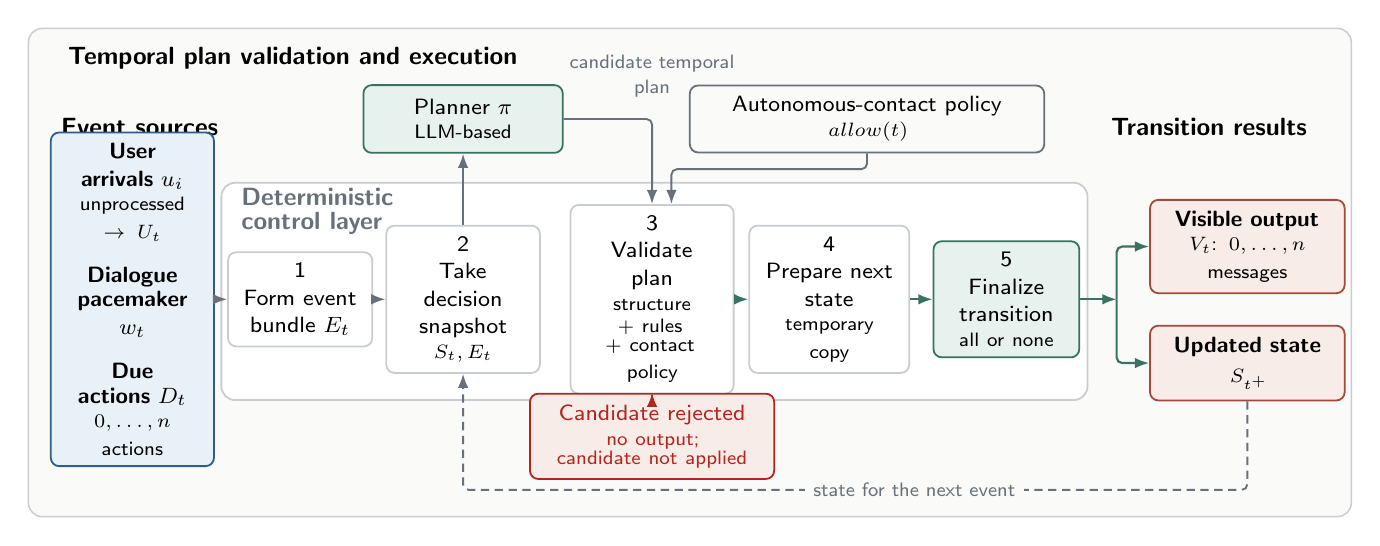
\begin{tikzpicture}[pai-figure]
\tikzset{
  pai-arch-box/.style={
    rounded corners=3pt,
    draw=paiBorder,
    fill=white,
    line width=0.65pt,
    minimum height=0.92cm,
    align=center,
    inner xsep=5pt,
    inner ysep=4pt
  },
  pai-source-box/.style={
    pai-arch-box,
    draw=paiUser,
    fill=paiUserLight,
    text width=1.72cm,
    minimum height=2.25cm
  },
  pai-control-box/.style={
    pai-arch-box,
    text width=1.48cm
  },
  pai-planner-box/.style={
    pai-arch-box,
    draw=paiDecision,
    fill=paiDecisionLight,
    text width=2.18cm,
    minimum height=0.86cm
  },
  pai-commit-box/.style={
    pai-arch-box,
    draw=paiDecision,
    fill=paiDecisionLight,
    text width=1.50cm
  },
  pai-state-box/.style={
    pai-arch-box,
    draw=paiAgent,
    fill=paiAgentLight,
    text width=2.12cm,
    minimum height=0.95cm
  },
  pai-output-box/.style={
    pai-arch-box,
    draw=paiAgent,
    fill=paiAgentLight,
    text width=2.12cm,
    minimum height=0.72cm
  },
  pai-policy-box/.style={
    pai-arch-box,
    draw=paiNeutral,
    fill=paiPanel,
    text width=4.15cm,
    minimum height=0.78cm
  },
  pai-reject-box/.style={
    pai-arch-box,
    draw=paiRevision,
    fill=paiAgentLight,
    text=paiRevision,
    text width=2.75cm,
    minimum height=0.76cm
  },
  pai-flow/.style={
    -{Latex[length=1.8mm]},
    draw=paiNeutral,
    line width=0.68pt,
    rounded corners=2pt
  },
  pai-accepted/.style={
    -{Latex[length=1.8mm]},
    draw=paiDecision,
    line width=0.78pt,
    rounded corners=2pt
  },
  pai-rejected/.style={
    -{Latex[length=1.8mm]},
    draw=paiRevision,
    line width=0.78pt
  }
}

\filldraw[pai-panel] (0,0) rectangle (16.8,6.20);
\node[pai-panel-title, anchor=west] at (0.38,5.82)
  {Temporal plan validation and execution};

\node[pai-panel-title, anchor=west] at (0.29,4.95) {Event sources};
\node[pai-source-box] (sources) at (1.32,2.76) {
  \textbf{User arrivals $u_i$}\\[-1pt]
  {\scriptsize unprocessed $\rightarrow U_t$}\\[6pt]
  \textbf{Dialogue}\\[-1pt]
  \textbf{pacemaker $w_t$}\\[6pt]
  \textbf{Due}\\[-1pt]
  \textbf{actions $D_t$}\\[-1pt]
  {\scriptsize $0,\ldots,n$ actions}
};

\filldraw[rounded corners=5pt, fill=white, draw=paiBorder, line width=0.65pt]
  (2.45,1.48) rectangle (13.45,4.24);
\node[pai-panel-title, text=paiNeutral, anchor=west, align=left] at (2.58,3.88)
  {Deterministic\\[-2pt]control layer};

\node[pai-control-box] (dispatch) at (3.45,2.76)
  {1\\Form event\\bundle $E_t$};
\node[pai-control-box, text width=1.60cm] (snapshot) at (5.52,2.76)
  {2\\Take decision\\snapshot\\[-1pt]{\scriptsize $S_t,E_t$}};
\node[pai-control-box, text width=1.72cm] (validate) at (7.92,2.76)
  {3\\Validate\\plan\\[1pt]{\scriptsize structure + rules\\[-3pt]+ contact policy}};
\node[pai-control-box, text width=1.68cm] (draft) at (10.17,2.76)
  {4\\Prepare next\\state\\[-1pt]{\scriptsize temporary copy}};
\node[pai-commit-box] (commit) at (12.42,2.76)
  {5\\Finalize\\transition\\[-1pt]{\scriptsize all or none}};

\node[pai-planner-box] (planner) at (5.52,5.05)
  {Planner $\pi$\\[-1pt]{\scriptsize LLM-based}};
\node[pai-policy-box] (policy) at (10.65,5.05)
  {\mbox{Autonomous-contact policy}\\[-1pt]
   {\scriptsize $\operatorname{allow}(t)$}};

\node[pai-panel-title, anchor=east] at (16.36,4.95) {Transition results};
\node[pai-output-box] (output) at (15.48,3.43) {
  \textbf{Visible output}\\[-1pt]
  {\scriptsize $V_t$: $0,\ldots,n$ messages}
};
\node[pai-state-box] (state) at (15.48,1.95) {
  \textbf{Updated state}\\[1pt]
  {\scriptsize $S_{t^+}$}
};

\node[pai-reject-box] (reject) at (7.92,1.02)
  {Candidate rejected\\[1pt]{\scriptsize no output;\\[-3pt]candidate not applied}};

\draw[pai-flow] (sources.east) -- (dispatch.west);
\draw[pai-flow] (dispatch.east) -- (snapshot.west);
\draw[pai-accepted] (validate.east) -- (draft.west);
\draw[pai-accepted] (draft.east) -- (commit.west);
\coordinate (resultfork) at (13.82,2.76);
\draw[pai-accepted] (commit.east) -- (resultfork);
\draw[pai-accepted] (resultfork) |- (output.west);
\draw[pai-accepted] (resultfork) |- (state.west);

\draw[pai-flow]
  (snapshot.north) -- (planner.south);
\draw[pai-flow]
  (planner.east) -- (7.92,5.05) -- (validate.north);
\node[pai-secondary, align=center] at (7.92,5.59)
  {candidate temporal\\plan};
\draw[pai-flow]
  (policy.south) -- ++(0,-0.20) -| ([xshift=7pt]validate.north);

\draw[pai-rejected] (validate.south) -- (reject.north);
\draw[pai-flow, densely dashed]
  (state.south) -- (15.48,0.34) -- (5.52,0.34) -- (snapshot.south);
\node[pai-secondary, fill=paiPanel, inner xsep=3pt] at (11.25,0.34)
  {state for the next event};

\end{tikzpicture}
}
  \caption{时序计划的验证与执行架构。该图从左至右表示一次完整的状态转移。
  每条 $u_i$ 记录一次独立的用户发送。在一次决策开始时，尚未由成功提交的计划处理的
  消息按到达顺序组成 $U_t$。该列表与对话起搏信号 $w_t$ 以及到期行动 $D_t$
  共同形成事件组合 $E_t$；到期行动是已经到达执行时点的未来行动。基于大语言
  模型的规划器 $\pi$ 读取当前状态 $S_t$ 和 $E_t$，然后提出候选时序计划。计划
  可以包含即时消息、新的未来行动、对现有队列的修改，以及对到期行动的处理
  决定。候选计划产生后，控制层按照固定规则完成验证和状态更新。它检查计划
  结构是否完整、计划是否仍基于当前状态、状态与队列是否保持一致。对于没有
  待处理用户输入时的消息发送，控制层还检查自主联系许可 $\operatorname{allow}(t)$。
  合法计划首先被应用到临时状态；只有全部检查均通过后，可见输出 $V_t$ 和下一状态
  $S_{t^+}$ 才会共同生效，否则二者均不生效。$V_t$ 可以包含零条、一条或多条
  消息。$S_{t^+}$ 保存更新后的历史、未来行动队列、起搏器状态和联系策略，并沿
  虚线路径进入下一事件。如果候选计划不满足上述执行条件，本次计划不会生效；
  系统不发送候选消息，也不应用候选计划提出的状态变化。未处理的输入与到期
  行动继续保留；控制层可另行更新重试时间，在后续决策中依据最新状态重新处理。}
  \Description{独立到达的用户消息、对话起搏信号和到期行动进入一个包含五个
  步骤的确定性控制层。控制层上方基于大语言模型的规划器读取包含当前状态的
  决策快照，并返回候选时序计划；自主联系策略也进入验证步骤。成功路径依次验证
  计划、准备临时的下一状态，并使可见输出和更新状态共同生效；虚线把该状态
  带入下一次决策。红色分支表示候选计划未被接受，不产生候选输出或应用候选变化；
  后续重试由独立的恢复规则安排。}
  \label{fig:architecture}
\end{figure*}

\subsection{交互示例}

图~\ref{fig:prototype} 以面试对话为例，将用户可见的消息与相应的未来
行动和决策状态并列呈现。在初始状态中，两条独立发送的用户消息进入同一次判断，产生
助手连续发送的两条消息、一项留待稍后发送的准备内容和一次较晚的重新判断。
用户随后告知面试已经取消，下一次决策会在两项未来意图执行前将其移除，并针对
更新后的情境自然作出回应。当日晚些时候，对话起搏事件尊重用户希望暂不讨论的
意愿并保持沉默；两天后的另一次起搏则在没有新用户输入的情况下主动发起关心。

\begin{figure*}[t]
  \centering
  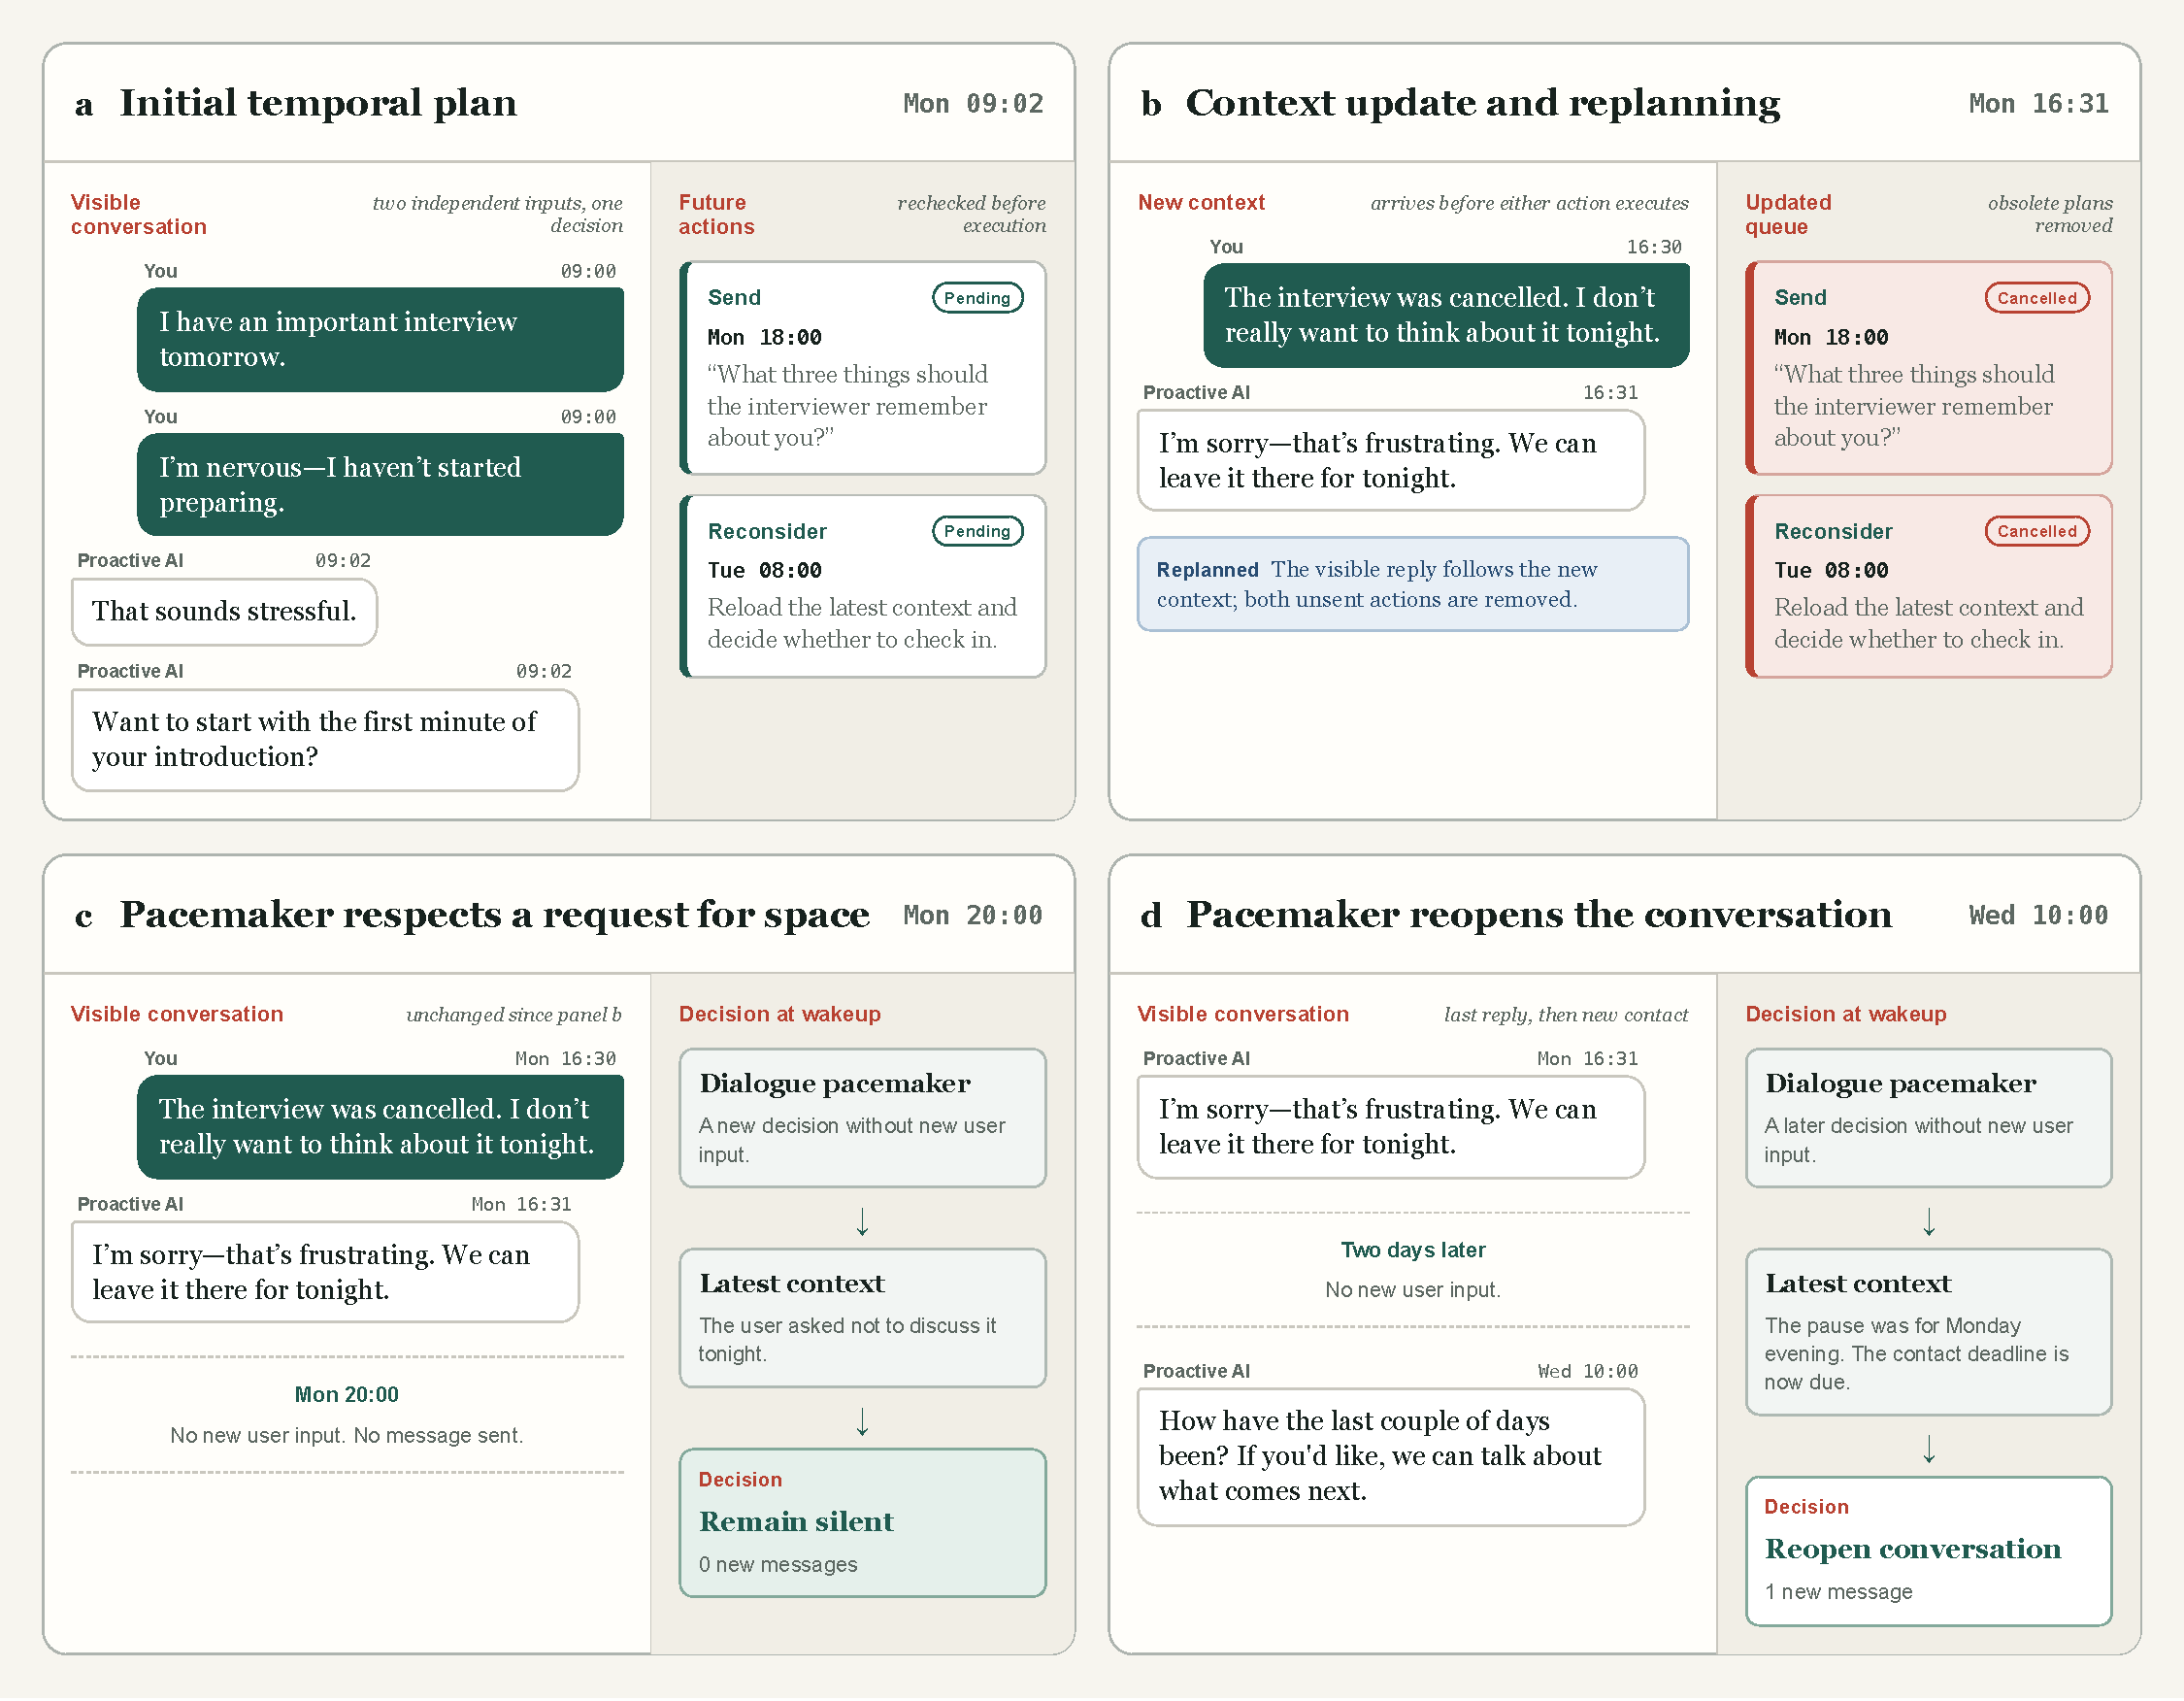
\includegraphics[width=\textwidth]{figures/prototype-inspection.pdf}
  \caption{时序对话交互示例。\textbf{a}，两条独立发送的用户消息进入同一次
  判断，产生两条即时消息，并创建两类未来行动：\emph{Send} 保存引号内的待发送
  原文，\emph{Reconsider} 仅保留稍后判断是否跟进的目的。\textbf{b}，用户告知面试已经取消后，两项尚未执行的行动
  在内部被取消，可见回复则自然回应新情境，而不向用户描述队列操作。\textbf{c}，当日晚些
  时候的对话起搏尊重用户希望暂不讨论的意愿，聊天记录保留此前的交流，但不新增
  消息。\textbf{d}，两天后，另一次对话起搏基于最新情境，在没有新用户输入的情况下
  主动发起关心，表现为时间间隔后出现的一条新聊天消息。聊天记录与对应的判断
  过程并列呈现。后两个
  状态共同说明，一次新的判断机会既可以产生沉默，也可以重新开启交流。}
  \Description{时序交互示例的四个状态。第一个状态显示两条即时助手消息和两项
  待执行的未来行动；第二个状态显示较晚到来的用户更新、自然的确认回复，以及
  两项未来行动在内部被取消；第三个状态并列显示未新增消息的既有聊天记录，以及
  当日晚间因用户希望暂不讨论而保持沉默的起搏决策；第四个状态显示此前最后一条
  回复、两天没有用户输入的间隔及随后主动发出的一条关心消息，并在旁边呈现
  对应的起搏决策。}
  \label{fig:prototype}
\end{figure*}

\section{讨论}

本文模型使对话的继续不再完全依赖用户再次发起请求。即使没有待发送消息或
预先安排的跟进，系统仍可在对话起搏时依据已有情境判断是否开启交流。它既
可以延续未完成事项，也可以在一次交流结束后提出新的话题。系统因此能够
分担记住未解决事项、选择跟进时点和重新发起对话的工作，为减轻持续协作中
用户的协调负担提供了可能。交互的连续性由此不必表现为持续发送消息，也可以
体现为暂时沉默之后的适时参与。

从这一角度看，面向长期协作的系统不仅需要保存过去的信息，还需要组织未来
的参与。记忆帮助系统理解此前发生了什么；时序计划则表示哪些事项值得稍后
关注，以及何时应当重新作出判断。二者相互补充：过去的情境为未来行动提供
依据，而未来行动又必须随着新信息被修订。系统因而可以保留跟进的意图，而
不必提前确定届时的表达。

例如，AI 导师可以在讲解结束后重新关注某个尚未解决的理解困难，根据学习者
后续的进展决定继续解释、调整练习或暂不介入；科学助手可以在等待实验结果
期间保留一个待重新检视的问题，并在新证据出现后决定是否继续分析或修正
建议。在这些场景中，系统的参与时机和方式应当随任务进展而调整。

除任务协作外，关系型智能体研究也将跨越多次交流的人机关系建立与维持视为
交互设计问题 \cite{bickmore2005relationships}。本文的时序组织方式可用于
陪伴型 AI 等面向日常交流与情感支持的系统。在这些场景中，拟人化不仅体现为语言风格，也体现为交流的主动性、
连续性与对情境变化的敏感性。系统可以在用户没有再次发问时，根据此前的交流主动表达关心，
并依据最新情况调整联系的时机和内容。例如，在得知用户的面试被取消后，系统
可以尊重其暂不讨论的意愿，撤销原有的面试提醒，并在稍后的适当时点重新询问
近况。这样的交互所追求的体贴，不只是措辞温暖，而是能够顾及用户当下的处境，
在主动联系与保留空间之间作出适当选择。

主动对话也为更一般的自主行为提供了研究切入点。Yang 等在 AI 科学家的研究中
区分了科研活动的发起与研究任务的执行，并讨论了 AI 能否承担科学“第一推动者”
（First Mover of Science）的角色~\cite{yang2023ai}。这一区分提示，自主完成
给定任务与自主发起活动是不同层面的能力。本文从持续对话出发，将没有新用户
请求时的重新判断，以及随情境变化修订未来行动，纳入可执行的时序模型。
这样的机制可作为研究更广泛自主交互的一项基础，其潜在扩展包括协作机器人的
高层任务规划。

例如，在已授权的实验室巡检任务中，机器人可以自主安排稍后前往某台设备
检查状态，并在执行前重新确认是否仍有必要。如果该项检查已由工作人员完成，
就取消尚未执行的巡视；如果通道暂时被占用，则推迟行动。这类扩展需要把
时序计划与环境感知、动作执行及安全控制机制结合，使重新获得判断机会与
实际执行物理动作保持区分。

综上，本文将是否参与、何时参与以及如何随情境修订参与计划纳入同一对话
过程。其意义不仅在于提供更自然的交流节奏，更在于为持续协作提供一种可
主动发起、可延后、可修改的时间组织方式。主动性的价值应体现为对用户需要
和共同活动的适时支持，而不是消息或动作数量的增加。

\section{结论}

本文提出 Proactive AI，一种以可重排时序消息队列为核心的主动式对话框架。
该框架将对话建模为连续的事件时间线，在同一模型下
表示沉默、多消息输出、延迟回复和主动发起。通过将尚未执行的对话行动表示为
可修改状态，并在执行前依据最新情境重新判断，该模型使未来表达能够被修订
或撤销，而非仅因预定时间到达便自动发送。形式化模型与开源研究原型为这一
交互范式提供了可执行基础。其意义不仅在于改变消息发送的节奏，更在于使 AI
能够在没有新请求时重新发起交流、持续关注未完成事项，并随情境变化调整
后续行动。由此，对话式 AI 可以从逐次响应走向持续且可修订的参与，为分担
长期人机协作中的跟进与协调工作提供机制支持。这种对未来参与的组织方式，
也为研究更广泛的自主交互提供了起点。

\renewcommand{\acksname}{致谢}
\begin{acks}
感谢博士期间的室友孙舒丰与作者就主动式对话 AI 的交互场景进行的
有益讨论。
\end{acks}

\bibliographystyle{ACM-Reference-Format}
\bibliography{references}

\clearpage
\appendix
\section{附图}
\label{app:supplementary-figures}
\setcounter{figure}{0}
\renewcommand{\theHfigure}{supp.\arabic{figure}}
\captionsetup[figure]{name=附图}

\begin{figure*}[ht]
  \centering
  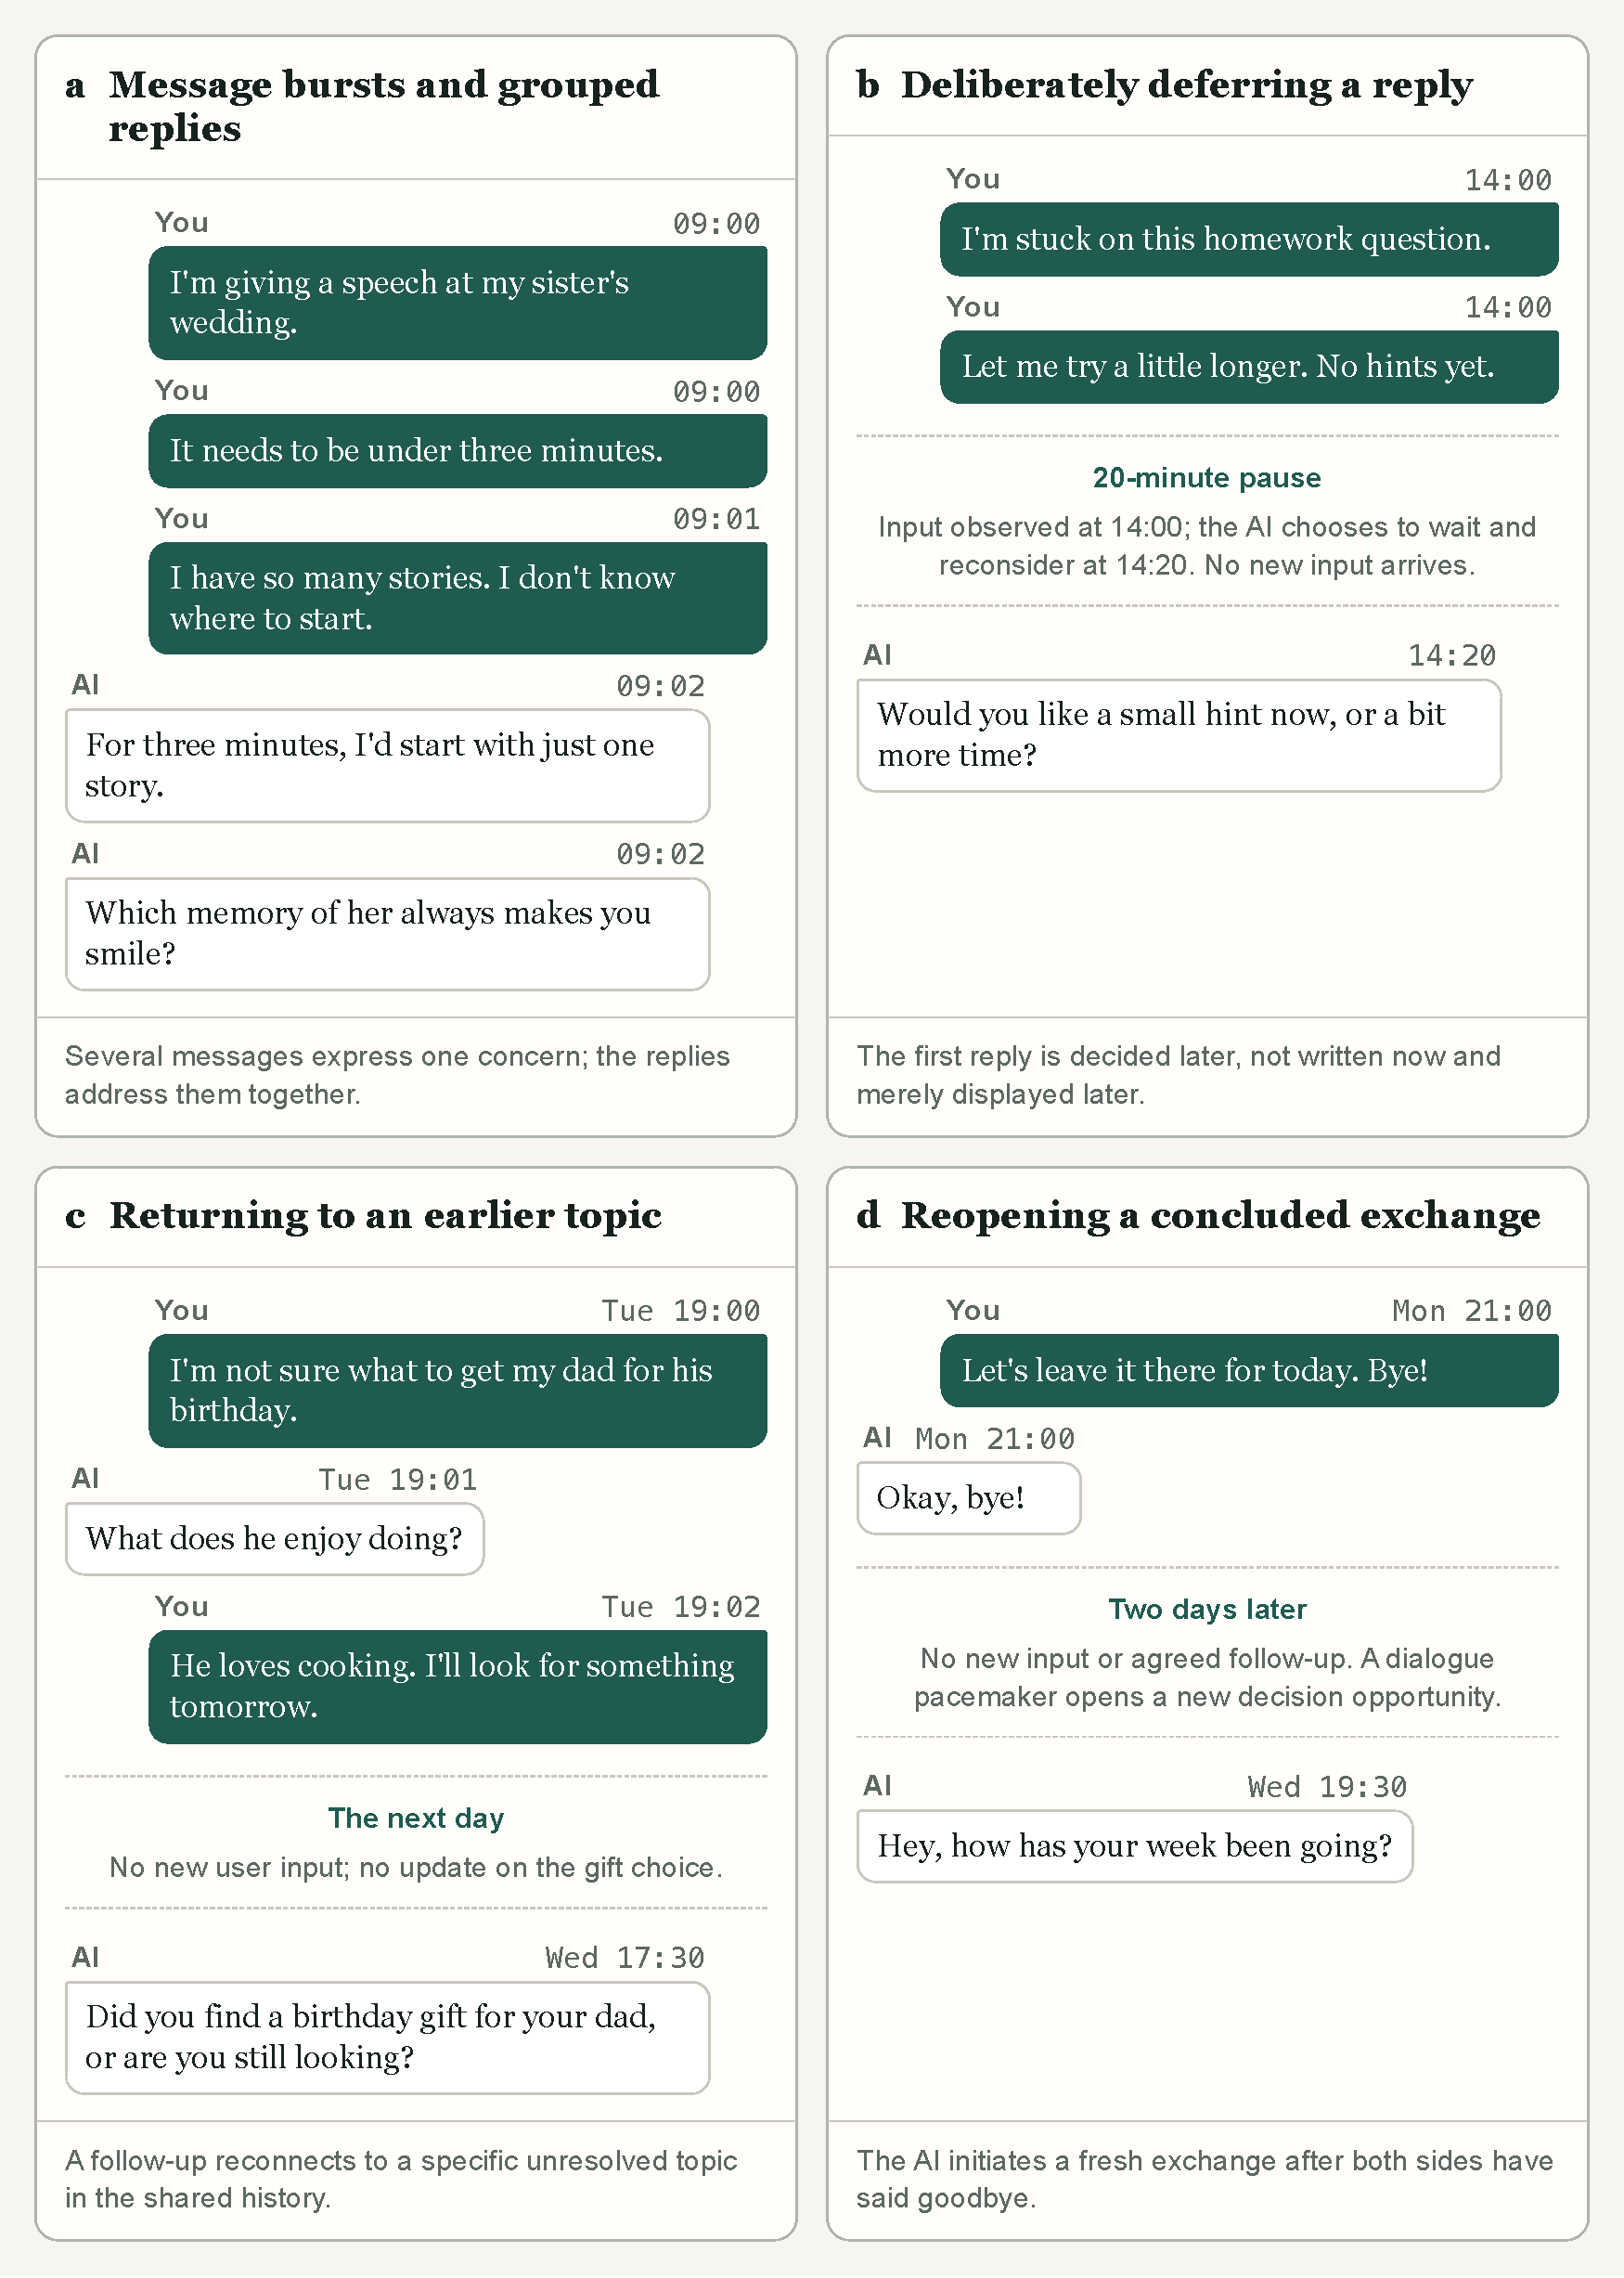
\includegraphics[width=\textwidth,height=0.78\textheight,keepaspectratio]{figures/dialogue-patterns.pdf}
  \caption{超越配对轮次的对话模式示例。
  \textbf{a}，连续输入与集中回应。多条用户消息共同表达一个问题，AI 连续
  发送多条消息集中回应，而非逐条配对回答。
  \textbf{b}，延迟首次回复。AI 在 14:00 已观察到用户输入，但暂不回应，直到
  14:20 才重新判断并生成首次回复。
  \textbf{c}，跨时段的话题跟进。AI 在一段时间后回到双方此前讨论过但尚未
  解决的话题，延续已有交流。
  \textbf{d}，道别后的主动发起。双方道别后，对话起搏器为 AI 提供新的判断
  机会，使其在没有新用户输入、也未约定后续联系的情况下主动开启交流。}
  \Description{四个带时间戳的聊天面板。面板 a 展示用户围绕一次简短婚礼致辞
  连续发送三条消息，AI 随后回复两条消息。面板 b 展示用户希望独立完成作业题，
  AI 主动等待二十分钟后首次回复。面板 c 展示为父亲挑选生日礼物的话题，以及
  AI 在次日对挑选进展的跟进。面板 d 展示双方道别后，AI 在两天后发起新的交流。
  用户消息靠右、采用深绿色气泡；AI 消息靠左、采用白色气泡。决策说明位于
  聊天气泡之外。}
  \label{fig:dialogue-patterns}
\end{figure*}

\end{document}
